% % Template for ICIP-2026 paper; to be used with:
% %          spconf.sty  - ICASSP/ICIP LaTeX style file, and
% %          IEEEbib.bst - IEEE bibliography style file.
% % --------------------------------------------------------------------------
% \documentclass{article}
% \usepackage{spconf,amsmath,amssymb,graphicx}
% % Bold italic math symbols (vectors/matrices)
% \usepackage{bm}
% % Chinese support (XeLaTeX)
% \usepackage{fontspec}
% \usepackage{xeCJK}
% % Hyperlinks for references (load near end of preamble)
% \usepackage{hyperref}
% \hypersetup{
%   colorlinks=true,
%   linkcolor=blue,
%   citecolor=blue,
%   urlcolor=blue,
%   bookmarksnumbered=true,
%   pdfstartview=FitH
% }
% % Prefer Noto CJK fonts; fallback to WenQuanYi if unavailable.
% \IfFontExistsTF{Noto Serif CJK SC}{
%   \setCJKmainfont{Noto Serif CJK SC}
% }{
%   \IfFontExistsTF{Noto Sans CJK SC}{
%     \setCJKmainfont{Noto Sans CJK SC}
%   }{
%     \IfFontExistsTF{WenQuanYi Zen Hei}{
%       \setCJKmainfont{WenQuanYi Zen Hei}
%     }{
%       \IfFontExistsTF{AR PL UMing CN}{
%         \setCJKmainfont{AR PL UMing CN}
%       }{
%         % Last resort: let XeTeX try system default (may still warn).
%         \setCJKmainfont{SimSun}
%       }
%     }
%   }
% }
% \IfFontExistsTF{WenQuanYi Zen Hei Mono}{\setCJKmonofont{WenQuanYi Zen Hei Mono}}{}
% % Better Chinese line breaking
% \XeTeXlinebreaklocale "zh"
% \XeTeXlinebreakskip = 0pt plus 1pt

% % Example definitions.
% % --------------------
% \def\x{{\bm x}}
% % NOTE: Avoid overriding \L (reserved command in LaTeX). Use \mathcal{L} directly.

% % Title.
% % ------
% \title{CoReGate: Counterfactual Reliability-Gated Fusion for Robust Multimodal Sentiment Analysis}
% %
% % Single address.
% % ---------------
% \name{\normalsize\shortstack{Pan Tang$^{1}$, Michele Nappi$^{2}$, Shaojing Song$^{3}$,\\
% Mingliang Gao$^{4}$, Hengyu Liu$^{5}$, Zhiqing Miao$^{6}$\sthanks{Corresponding author: Zhiqiang Miao.},\\
% Xuying Zheng$^{7}$\sthanks{Co-corresponding author: Xuying Zheng.}}}
% \address{\normalsize\shortstack{\textsuperscript{1}School of Communication and Information Engineering, Shanghai University, China\\
% \textsuperscript{2}University of Salerno, Italy\\
% \textsuperscript{3}School of Computer and Informational Engineering, Shanghai Polytechnic University, China\\
% \textsuperscript{4}School of Electrical and Electronic Engineering, Shandong University of Technology, China\\
% \textsuperscript{5}Department of Computer Science, Aalborg University, Denmark\\
% \textsuperscript{6}School of Information and Electronic Engineering, East China Normal University, China\\
% \textsuperscript{7}School of Life Sciences, Tsinghua University, China\\
% \texttt{ptang@shu.edu.cn, mnappi@unisa.it, sjsong@sspu.edu.cn, mlgao@sdut.edu.cn,}\\
% \texttt{heli@cs.aau.dk, 52275904009@stu.ecnu.edu.cn, zhengxy20@mails.tsinghua.edu.cn}}}










% Template for ICIP-2026 paper; to be used with:
%          spconf.sty  - ICASSP/ICIP LaTeX style file, and
%          IEEEbib.bst - IEEE bibliography style file.
% --------------------------------------------------------------------------
\documentclass{article}
\usepackage{spconf,amsmath,graphicx}
\usepackage{graphicx}%
\usepackage{multirow}%
\usepackage{amsmath,amssymb,amsfonts}%
\usepackage{amsthm}%
\usepackage{mathrsfs}%
\usepackage[title]{appendix}%
\usepackage{xcolor}%
\usepackage{textcomp}%
\usepackage{manyfoot}%
\usepackage{booktabs}%
\usepackage{algorithm}%
\usepackage{algorithmicx}%
\usepackage{algpseudocode}%
\usepackage{listings}%
\usepackage{url} % 必须加载
\usepackage{bm} % for \bm{...} in equations
% Example definitions.
% --------------------
\def\x{{\mathbf x}}
% NOTE: avoid overriding \L (reserved command in LaTeX). Use \mathcal{L} directly.

% Title.
% ------
\title{CoReGate: Counterfactual Reliability-Gated Fusion for Robust Multimodal Sentiment Analysis}

% spconf's \maketitle typesets \name/\address inside a tabular cell; prefer
% \shortstack to safely use line breaks here.
\name{\normalsize\shortstack{
Pan Tang$^{1}$, Michele Nappi$^{2}$, Shaojing Song$^{3}$, Mingliang Gao$^{4}$,\\
Hengyu Liu$^{5}$, Zhiqing Miao$^{6}$\sthanks{Corresponding author: Zhiqing Miao (52275904009@stu.ecnu.edu.cn).}, Xuying Zheng$^{7}$\sthanks{Co-corresponding author: Xuying Zheng (zhengxy20@mails.tsinghua.edu.cn).}
}}
\address{\normalsize\shortstack{
$^{1}$ School of Communication and Information Engineering, Shanghai University, China\\
$^{2}$ Department of Computer Science, University of Salerno, Italy\\
$^{3}$ School of Computer and Informational Engineering, Shanghai Polytechnic University, China\\
$^{4}$ School of Electrical and Electronic Engineering, Shandong University of Technology, China\\
$^{5}$ Department of Computer Science, Aalborg University, Denmark\\
$^{6}$ School of Information and Electronic Engineering, East China Normal University, China\\
$^{7}$ School of Life Sciences, Tsinghua University, China
}}

\begin{document}
%\ninept
%
\maketitle
%
\begin{abstract}
In multimodal sentiment analysis, text is often more reliable than audio and vision. However, audiovisual signals can be noisy, missing, or semantically inconsistent with the text (e.g., sarcasm). In such cases, straightforward fusion may inject unreliable evidence and amplify prediction errors. We propose CoReGate (Counterfactual Reliability-Gated Fusion), which models non-textual modalities as marginal corrections to a text-backbone predictor. Multi-branch predictors explicitly estimate the marginal contributions from audio and vision, while sample-wise reliability gates selectively inject these corrections. This design suppresses unreliable increments when non-textual modalities are unreliable, improving prediction stability. Experiments on CMU-MOSI and CMU-MOSEI demonstrate competitive performance on standard metrics and improved robustness under missing-modality stress tests.
\end{abstract}
%
\begin{keywords}
Multimodal sentiment analysis, counterfactual contribution, reliability gating, robust fusion
\end{keywords}
%
\section{INTRODUCTION}
\label{sec:intro}

Multimodal sentiment analysis (MSA) predicts sentiment polarity or intensity by integrating text, audio, and vision cues~\cite{zhu2024review}. While fusion can be beneficial, non-textual modalities are often noisy, missing, or semantically inconsistent with text (e.g., sarcasm), which may inject unreliable evidence and destabilize predictions~\cite{williams2018dnn,wang2022cross}. Fig.~\ref{fig:intro_motivation} illustrates this issue.

\begin{figure}[t]
  \centering
  \includegraphics[width=0.98\linewidth]{figures/fig1}
  \caption{Motivation for robust multimodal fusion. When audio and vision are noisy or semantically conflicting with text (e.g., sarcasm), simple fusion may amplify prediction errors.}
  \label{fig:intro_motivation}
\end{figure}

\begin{figure*}[t]
  \centering
  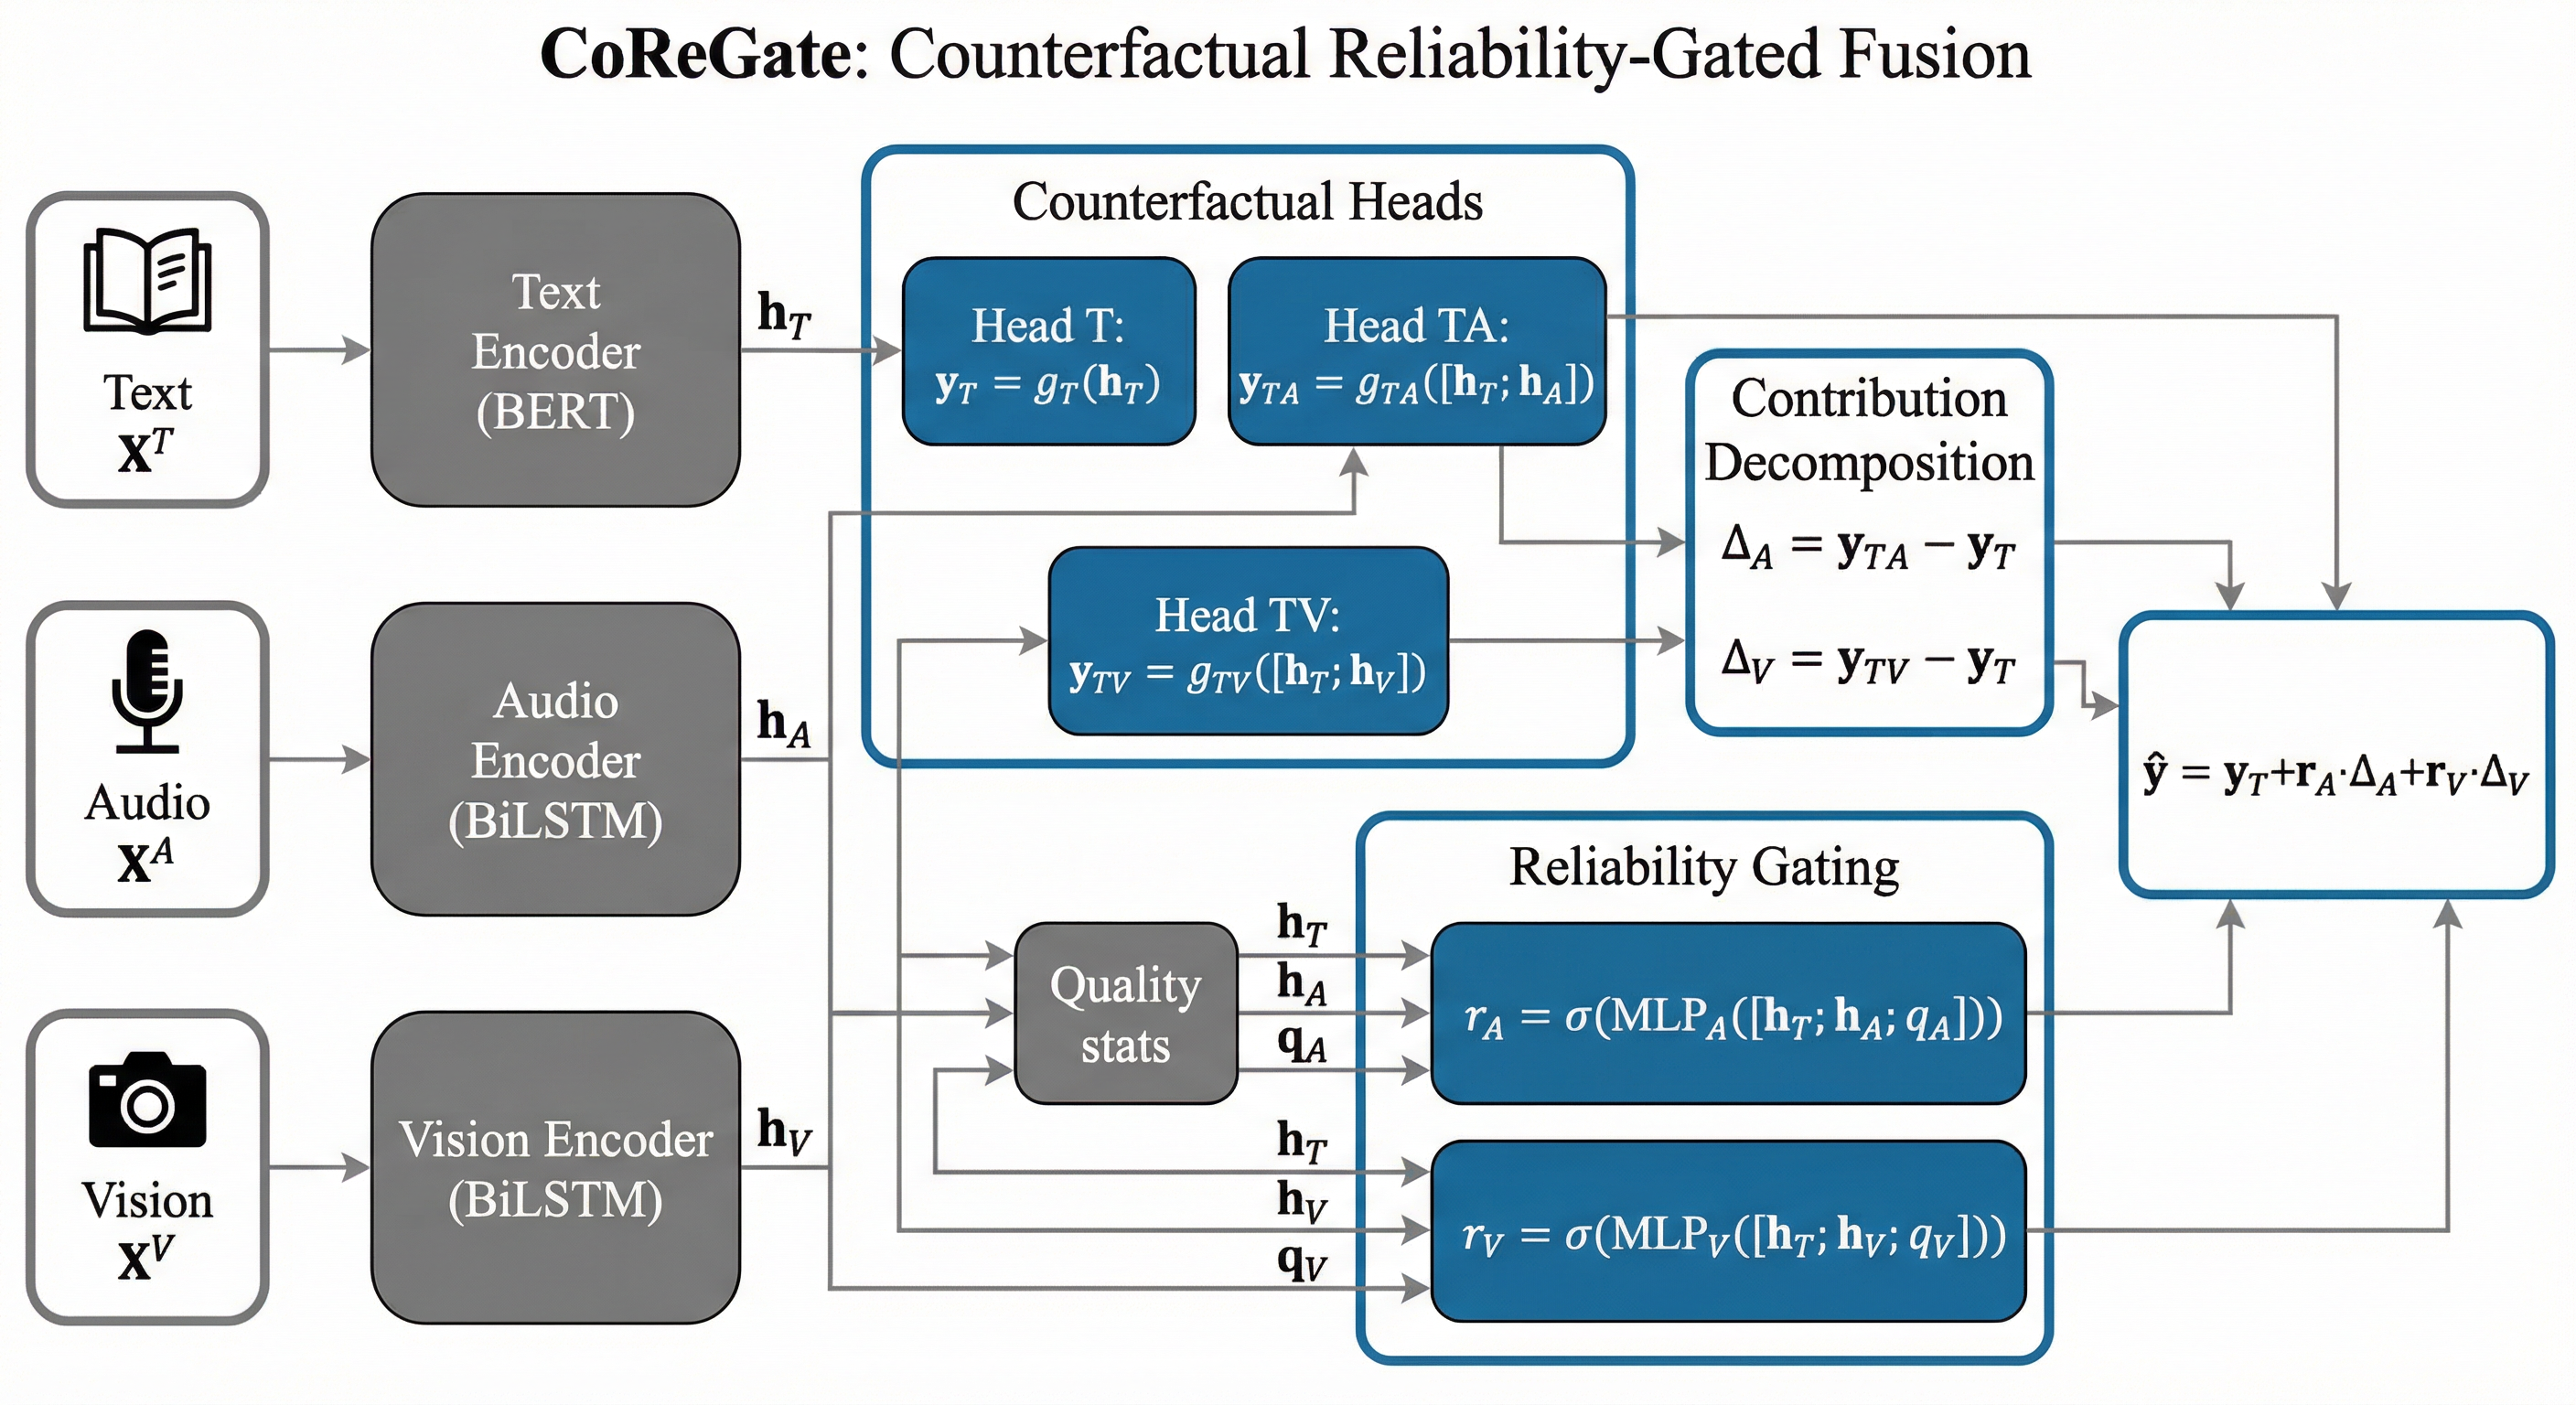
\includegraphics[width=0.98\textwidth]{figures/fig2}
  \caption{Overview of CoReGate. Text is treated as a backbone predictor. Audio and vision provide marginal increments (\(\Delta_{\mathrm{A}},\Delta_{\mathrm{V}}\)) estimated by counterfactual heads and injected by sample-wise reliability gates (\(r_{\mathrm{A}},r_{\mathrm{V}}\)).}
  \label{fig:framework}
\end{figure*}

Prior work explores a broad spectrum of fusion and representation strategies, including early/intermediate/late fusion and decision-level combination~\cite{williams2018dnn} and simple early fusion baselines for video emotion/sentiment modeling~\cite{williams2018recognizing}, dominant-modality completion~\cite{huang2023dominant}, explicit interaction modeling (e.g., tensor fusion)~\cite{zadeh2017tensor,liu2018efficient}, sequential/memory/graph-based fusion~\cite{zadeh2018memory,zadeh2018multimodal,hu2024graph}, factorized/invariant representations~\cite{tsai2019learning,hazarika2020misa}, text-centric enhancement for unaligned settings~\cite{wang2022cross,wang2023tetfn,li2025caetfn}, and self-supervised multi-task learning~\cite{yu2021learning}. Robustness to noise/missing modalities has also been studied via incomplete-modality learning and contrastive objectives~\cite{jiang2025boosting,wang2025contrastive,zhuang2025multi}, and related progress appears in aspect-based settings~\cite{wang2024dual}.

However, many methods still lack an explicit, sample-wise mechanism to control how much non-textual information should be trusted when audio/vision are noisy, missing, or conflicting with text. We therefore pursue a text-backbone design with controllable incremental injection of non-textual evidence.

CoReGate (Counterfactual Reliability-Gated Fusion) models audio and vision as marginal corrections to a text prediction. It estimates each modality's correction by multi-branch counterfactual differences, and then selectively injects them through sample-wise reliability gates, improving stability under noisy, missing, or conflicting non-text modalities.

The main contributions are summarized as follows:
\begin{itemize}
  \item We propose a robust fusion framework based on counterfactual contribution decomposition and reliability gating, where non-textual modalities are modeled as explicit increments to a text backbone.
  \item Experiments on CMU-MOSI and CMU-MOSEI demonstrate competitive performance on standard metrics and improved robustness under missing-modality stress tests.
\end{itemize}

\section{PROPOSED METHOD}
\label{sec:method}

This section introduces a robust fusion framework based on counterfactual contribution decomposition and reliability gating. The text branch serves as the backbone predictor, while audio and vision are treated as incremental evidence to correct the text output. Three prediction branches (\(\mathrm{T}\), \(\mathrm{TA}\), and \(\mathrm{TV}\)) are trained to derive marginal contributions. Sample-wise gates then control how these contributions are injected, improving robustness when non-textual modalities are noisy or conflicting.

As shown in Fig.~\ref{fig:framework}, the three modalities are encoded into \(\bm{h}_{\mathrm{T}},\bm{h}_{\mathrm{A}},\bm{h}_{\mathrm{V}}\). Three branch predictors output \(y_{\mathrm{T}},y_{\mathrm{TA}},y_{\mathrm{TV}}\). Marginal contributions \(\Delta_{\mathrm{A}},\Delta_{\mathrm{V}}\) are computed and injected through reliability coefficients \(r_{\mathrm{A}},r_{\mathrm{V}}\) predicted by a gating network from representation cues and quality statistics \((\bm{q}_{\mathrm{A}},\bm{q}_{\mathrm{V}})\). The final output selectively injects increments to suppress unreliable non-textual evidence.

\subsection{Problem Formulation}
\label{ssec:form}

The three-modal input is represented as sequential features \(\bm{X}^{(\mathrm{T})},\bm{X}^{(\mathrm{A})},\bm{X}^{(\mathrm{V})}\). Let \(\mathrm{T},\mathrm{A},\mathrm{V}\) denote modality indices. An encoder \(E_m(\cdot)\) maps modality \(m\in\{\mathrm{T},\mathrm{A},\mathrm{V}\}\) to a sentence-level vector \(\bm{h}_m = E_m(\bm{X}^{(m)})\). For any modality subset \(\mathcal{S}\subseteq\{\mathrm{T},\mathrm{A},\mathrm{V}\}\), a branch prediction is defined as

\begin{equation}
y_{\mathcal{S}} = g_{\mathcal{S}}\!\left(f_{\mathcal{S}}\big(\{\bm{h}_m\}_{m\in \mathcal{S}}\big)\right),\quad \mathcal{S}\in\{\mathrm{T},\mathrm{TA},\mathrm{TV}\}.
\end{equation}
where \(f_{\mathcal{S}}(\cdot)\) is the fusion operator of branch \(\mathcal{S}\) (concatenation followed by a multilayer perceptron (MLP) in this work), and \(g_{\mathcal{S}}(\cdot)\) is the corresponding regression head that outputs the scalar \(y_{\mathcal{S}}\). In the following, \(y_{\mathrm{T}}\) is used as the text-backbone output, and the other branches are used to construct controllable incremental contributions.

\subsection{Encoders and Representations}
\label{ssec:enc}
Text, audio, and vision are represented as sequence inputs. Audio and vision may be unaligned with text, and padded time steps are handled via valid lengths or masks. The text encoder is a pretrained language model; the sentence-level representation \(\bm{h}_{\mathrm{T}}\) is taken from the classification token ([CLS]) hidden state. For audio and vision, lightweight temporal encoders model frame-level features and then aggregate them into sentence-level vectors \(\bm{h}_{\mathrm{A}},\bm{h}_{\mathrm{V}}\). The aggregation uses text-guided attentive pooling, where the text representation serves as the query to select semantically relevant segments from the unaligned audio/visual sequences. The resulting \(\bm{h}_{\mathrm{T}},\bm{h}_{\mathrm{A}},\bm{h}_{\mathrm{V}}\) are used for the three-branch predictions and reliability gating.

\subsection{Counterfactual Contribution Decomposition}
\label{ssec:cf}

Many fusion methods rely on implicit attention or alignment to balance modalities, and an operational, quantifiable definition of ``modality contribution'' is often lacking. With only sequence-level sentiment supervision, it is also difficult to learn when a modality should be trusted or suppressed. Here, a modality contribution is defined as the prediction difference caused by adding that modality while keeping the others unchanged. This gives the contribution an explicit counterfactual meaning and enables direct estimation via multi-branch predictions.

Specifically, text is treated as the backbone, and audio/vision are treated as optional correction signals. Let \(y_{\mathrm{T}}\) denote the text-only prediction, and let \(y_{\mathrm{TA}}\) and \(y_{\mathrm{TV}}\) denote the text+audio and text+vision predictions, respectively. The marginal contributions are defined as
\begin{equation}
\begin{aligned}
\Delta_{\mathrm{A}} &= y_{\mathrm{TA}}-y_{\mathrm{T}}, \\
\Delta_{\mathrm{V}} &= y_{\mathrm{TV}}-y_{\mathrm{T}}.
\end{aligned}
\end{equation}
Intuitively, \(\Delta_{\mathrm{A}}\) and \(\Delta_{\mathrm{V}}\) quantify the net corrections of audio and vision relative to the text prediction. This decomposition turns fusion gains into computable difference terms and shifts fusion from implicit feature reweighting to explicit modeling of incremental evidence. Based on these increments, reliability gating performs sample-wise selective injection, improving training stability and robustness.

\subsection{Reliability-Gated Fusion}
\label{ssec:gate}

In real data, audio or vision can be noisy, missing, or semantically inconsistent with text. Injecting all contributions indiscriminately may systematically bias predictions. Therefore, sample-wise gate coefficients \(r_{\mathrm{A}}, r_{\mathrm{V}}\in[0,1]\) are learned to modulate each increment according to its estimated reliability. The final prediction is
\begin{equation}
\hat{y} = y_{\mathrm{T}} + r_{\mathrm{A}}\Delta_{\mathrm{A}} + r_{\mathrm{V}}\Delta_{\mathrm{V}}.
\end{equation}
When a modality is unreliable, a smaller gate suppresses its increment, making the output closer to the text backbone. When complementary information is present, the gate allows injection to correct the output. To align the gates with the notion of reliability, the gating network is built on representation cues and modality-quality statistics. Since branch fusion uses concatenation, the gate inputs are constructed from \(\bm{h}_{\mathrm{T}},\bm{h}_{\mathrm{A}},\bm{h}_{\mathrm{V}}\) and the quality statistics:
\begin{equation}
\begin{aligned}
\bm{z}_{\mathrm{A}} &= \big[\bm{h}_{\mathrm{T}};\bm{h}_{\mathrm{A}};\bm{q}_{\mathrm{A}} \big], \\
\bm{z}_{\mathrm{V}} &= \big[\bm{h}_{\mathrm{T}};\bm{h}_{\mathrm{V}};\bm{q}_{\mathrm{V}} \big],
\end{aligned}
\end{equation}
The gate coefficients are predicted by MLPs:
\begin{equation}
\begin{aligned}
r_{\mathrm{A}} &= \sigma(\mathrm{MLP}_{\mathrm{A}}(\bm{z}_{\mathrm{A}})), \\
r_{\mathrm{V}} &= \sigma(\mathrm{MLP}_{\mathrm{V}}(\bm{z}_{\mathrm{V}})).
\end{aligned}
\end{equation}
where \(\sigma(\cdot)\) is the sigmoid function. Here, \(\bm{h}_{\mathrm{T}}\) is the text representation, and \(\bm{h}_{\mathrm{A}},\bm{h}_{\mathrm{V}}\) are audio/visual contextual representations conditioned on text. \(\bm{q}_{\mathrm{A}},\bm{q}_{\mathrm{V}}\) are low-dimensional sample-wise quality statistics that provide reliability cues. In our implementation, the \(L_2\) norm of frame-level features is computed over valid time steps, and its mean, standard deviation, and valid ratio form \(\bm{q}\in\mathbb{R}^{3}\).

Instead of learning weights directly on fused features, gating is applied to the contribution differences, making the gates closer to ``whether the modality provides reliable incremental evidence.'' The overall forward computation and objective are summarized in Algorithm~\ref{alg:coregate}.

\begin{algorithm}[t]
\caption{CoReGate forward computation and training objective.}
\label{alg:coregate}
\begin{algorithmic}[1]
\Require A training sample \((\bm{X}^{(\mathrm{T})}, \bm{X}^{(\mathrm{A})}, \bm{X}^{(\mathrm{V})}, y)\); encoders \(E_{\mathrm{T}},E_{\mathrm{A}},E_{\mathrm{V}}\); heads \(g_{\mathrm{T}},g_{\mathrm{TA}},g_{\mathrm{TV}}\); gating MLPs \(\mathrm{MLP}_{\mathrm{A}},\mathrm{MLP}_{\mathrm{V}}\); loss \(\ell(\cdot,\cdot)\); branch weight \(\lambda\)
\Ensure Prediction \(\hat{y}\) and training loss \(\mathcal{L}\)
\State \(\bm{h}_{\mathrm{T}} \gets E_{\mathrm{T}}(\bm{X}^{(\mathrm{T})})\)
\State \(\bm{h}_{\mathrm{A}} \gets E_{\mathrm{A}}(\bm{X}^{(\mathrm{A})})\), \(\bm{h}_{\mathrm{V}} \gets E_{\mathrm{V}}(\bm{X}^{(\mathrm{V})})\)
\State \(y_{\mathrm{T}} \gets g_{\mathrm{T}}(\bm{h}_{\mathrm{T}})\)
\State \(y_{\mathrm{TA}} \gets g_{\mathrm{TA}}([\bm{h}_{\mathrm{T}};\bm{h}_{\mathrm{A}}])\)
\State \(y_{\mathrm{TV}} \gets g_{\mathrm{TV}}([\bm{h}_{\mathrm{T}};\bm{h}_{\mathrm{V}}])\)
\State \(\Delta_{\mathrm{A}} \gets y_{\mathrm{TA}} - y_{\mathrm{T}}\), \(\Delta_{\mathrm{V}} \gets y_{\mathrm{TV}} - y_{\mathrm{T}}\)
\State \(\bm{q}_{\mathrm{A}} \gets \mathrm{QualityStats}(\bm{X}^{(\mathrm{A})})\) \Comment{e.g., mean/std/valid-ratio of frame-wise \(L_2\) norms}
\State \(\bm{q}_{\mathrm{V}} \gets \mathrm{QualityStats}(\bm{X}^{(\mathrm{V})})\)
\State \(r_{\mathrm{A}} \gets \sigma(\mathrm{MLP}_{\mathrm{A}}([\bm{h}_{\mathrm{T}};\bm{h}_{\mathrm{A}};\bm{q}_{\mathrm{A}}]))\)
\State \(r_{\mathrm{V}} \gets \sigma(\mathrm{MLP}_{\mathrm{V}}([\bm{h}_{\mathrm{T}};\bm{h}_{\mathrm{V}};\bm{q}_{\mathrm{V}}]))\)
\State \(\hat{y} \gets y_{\mathrm{T}} + r_{\mathrm{A}}\Delta_{\mathrm{A}} + r_{\mathrm{V}}\Delta_{\mathrm{V}}\)
\State \(\mathcal{L} \gets \ell(\hat{y},y) + \lambda\big(\ell(y_{\mathrm{T}},y) + \ell(y_{\mathrm{TA}},y) + \ell(y_{\mathrm{TV}},y)\big)\)
\State \Return \((\hat{y}, \mathcal{L})\)
\end{algorithmic}
\end{algorithm}

\begin{table*}[t]
  \centering
\caption{Main results on CMU-MOSI and CMU-MOSEI. Acc2/F1 is reported as Has0/Non0 (\%).}
  \label{tab:main}
  \small
  \begin{tabular}{l|ccccc|ccccc}
    \hline
    & \multicolumn{5}{c|}{\textbf{CMU-MOSI}} & \multicolumn{5}{c}{\textbf{CMU-MOSEI}} \\
    \hline
    Models & MAE$\downarrow$ & Corr$\uparrow$ & Acc7$\uparrow$ & Acc2$\uparrow$ & F1$\uparrow$ & MAE$\downarrow$ & Corr$\uparrow$ & Acc7$\uparrow$ & Acc2$\uparrow$ & F1$\uparrow$ \\
    \hline
    EF-LSTM~\cite{williams2018recognizing} & 0.956 & 0.658 & 32.5 & 78.1/79.3 & 78.2/79.4 & 0.593 & 0.689 & 50.0 & 78.2/81.7 & 78.7/81.7 \\
    LF-DNN~\cite{williams2018dnn} & 0.992 & 0.650 & 33.2 & 76.5/77.7 & 76.6/77.9 & 0.557 & 0.728 & 53.1 & \textbf{83.6}/83.7 & 83.3/83.1 \\
    TFN~\cite{zadeh2017tensor} & 0.988 & 0.640 & 35.6 & 75.1/76.1 & 75.1/76.2 & 0.565 & 0.725 & 52.7 & 80.4/83.4 & 80.9/83.4 \\
    LMF~\cite{liu2018efficient} & 0.981 & 0.637 & 36.0 & 75.4/76.2 & 75.4/76.3 & 0.562 & 0.739 & 51.5 & 81.8/83.9 & 82.1/83.8 \\
    MFN~\cite{zadeh2018memory} & 0.938 & 0.669 & 35.9 & 77.0/78.9 & 77.6/78.9 & 0.568 & 0.726 & 50.7 & 82.2/84.0 & 82.3/83.8 \\
    MFM~\cite{tsai2019learning} & 0.899 & 0.673 & 37.8 & 78.9/80.2 & 78.8/80.1 & 0.573 & 0.727 & 51.0 & 81.7/83.6 & 82.1/83.6 \\
    Graph-MFN~\cite{zadeh2018multimodal} & 0.886 & 0.693 & 37.6 & 79.6/81.0 & 79.4/80.8 & 0.562 & 0.725 & 52.1 & 83.3/83.4 & 83.1/82.8 \\
    MISA~\cite{hazarika2020misa} & 0.805 & 0.765 & 40.2 & 81.6/83.2 & 81.6/83.3 & 0.547 & 0.759 & 51.9 & 82.8/84.9 & 83.0/84.8 \\
    Self-MM~\cite{yu2021learning} & 0.726 & 0.784 & \textbf{48.0} & 82.5/84.5 & 82.5/84.5 & 0.539 & 0.765 & 52.8 & 74.8/82.0 & 76.0/82.3 \\
    TETFN~\cite{wang2023tetfn} & 0.731 & 0.790 & 45.2 & 80.9/82.8 & 80.9/82.8 & 0.546 & 0.762 & 53.9 & 80.6/85.1 & 81.1/85.1 \\
    MECAM~\cite{wang2025contrastive} & 0.730 & 0.788 & 45.5 & 81.8/83.5 & 81.7/83.4 & 0.535 & 0.770 & 53.8 & 81.8/85.5 & 82.0/85.2 \\
    CENET~\cite{wang2022cross} & 0.739 & 0.789 & 43.6 & 82.1/83.8 & 82.0/83.9 & \textbf{0.529} & 0.775 & \textbf{54.2} & 82.4/85.8 & 82.7/85.6 \\
    \textbf{Ours} & \textbf{0.707} & \textbf{0.794} & 47.7 & \textbf{82.8}/\textbf{84.8} & \textbf{82.7}/\textbf{84.8} & \textbf{0.529} & \textbf{0.777} & 53.1 & 83.3/\textbf{85.9} & \textbf{83.6}/\textbf{85.7} \\
    \hline
  \end{tabular}
\end{table*}


\subsection{Training Objective}
\label{ssec:loss}

The overall objective is included in Algorithm~\ref{alg:coregate}. The main task uses MAE (L1) regression loss. To stabilize branch learning and avoid branch collapse (e.g., \(\mathrm{TA}\) and \(\mathrm{TV}\) failing to learn meaningful increments, making \(\Delta_{\mathrm{A}},\Delta_{\mathrm{V}}\) noisy), auxiliary supervision is applied to the three branch outputs \(y_{\mathrm{T}},y_{\mathrm{TA}},y_{\mathrm{TV}}\) in addition to supervising the final prediction \(\hat{y}\). With a branch-loss weight \(\lambda\ge0\), the total objective is
% \begin{equation}
% \mathcal{L} = \mathcal{L}_{\hat{y}} + \lambda\left(\mathcal{L}_{\mathrm{T}} + \mathcal{L}_{\mathrm{TA}} + \mathcal{L}_{\mathrm{TV}}\right),
% \end{equation}
% where \(\mathcal{L}_{\hat{y}}\) supervises \(\hat{y}\), and \(\mathcal{L}_{\mathrm{T}}, \mathcal{L}_{\mathrm{TA}}, \mathcal{L}_{\mathrm{TV}}\) supervise \(y_{\mathrm{T}}, y_{\mathrm{TA}}, y_{\mathrm{TV}}\), respectively. This design improves the learnability of \(\Delta_{\mathrm{A}},\Delta_{\mathrm{V}}\). Without supervision on \(\mathrm{TA}\) and \(\mathrm{TV}\), the differences may become noisy and weaken the gating mechanism.
\begin{equation}
\mathcal{L} = \mathcal{L}_{\hat{y}} + \lambda\left(\mathcal{L}_{\mathrm{T}} + \mathcal{L}_{\mathrm{TA}} + \mathcal{L}_{\mathrm{TV}}\right),
\end{equation}
where $\mathcal{L}_{\hat{y}}$ supervises $\hat{y}$, and $\mathcal{L}_{\mathrm{T}}$, $\mathcal{L}_{\mathrm{TA}}$, $\mathcal{L}_{\mathrm{TV}}$ supervise $y_{\mathrm{T}}$, $y_{\mathrm{TA}}$, $y_{\mathrm{TV}}$, respectively. This design improves the learnability of $\Delta_{\mathrm{A}},\Delta_{\mathrm{V}}$. Without supervision on $\mathrm{TA}$ and $\mathrm{TV}$, the differences may become noisy and weaken the gating mechanism.

\section{EXPERIMENTAL RESULTS}
\label{sec:exp}

\subsection{Dataset and Metrics}
\label{ssec:dataset}

We evaluate sentiment regression on CMU-MOSI and CMU-MOSEI using standard splits and protocols. We report MAE, Pearson correlation (Corr), Acc7, and binary Acc2/F1 under Has0/Non0 settings (threshold at 0; Non0 excludes neutral samples). All percentages are reported in \%.

\subsection{Implementation Details}
\label{ssec:impl}

We use publicly released unaligned features (maximum lengths: 50/500/375 for text/audio/vision). The text encoder is \textit{BERT-base-uncased} and is fine-tuned end-to-end. Training uses Adam with MAE (L1) loss, learning rate \(1\times10^{-5}\), weight decay \(1\times10^{-4}\), gradient clipping at 2.0, and batch size 64. The best checkpoint is selected by validation loss, with early stopping if no improvement is observed for 8 epochs. All experiments are conducted on Ubuntu 22.04.5 with PyTorch 2.10.0 (CUDA 12.8) on an NVIDIA GeForce RTX 4090 (24GB) GPU and an AMD EPYC 9654 CPU.

\subsection{Evaluation of Our Method}
\label{ssec:main}

Table~\ref{tab:main} reports the main results on MOSI and MOSEI. Overall, the proposed method achieves competitive performance on both datasets and reaches the best or tied-best results on several key metrics.

On CMU-MOSI, the method achieves the best MAE and Corr, and also performs best under both Has0 and Non0 settings for binary Acc2/F1. Compared with a strong baseline CENET~\cite{wang2022cross}, MAE improves from 0.739 to 0.707 and Corr improves from 0.789 to 0.794, supporting the benefit of gating incremental non-textual evidence on top of a text backbone. The best Acc7 is achieved by Self-MM~\cite{yu2021learning}; our Acc7 (47.7) is close and remains competitive.

On CMU-MOSEI, the method achieves a slightly lower MAE and a higher Corr than CENET~\cite{wang2022cross}, while remaining competitive on Acc7. It also attains the best Non0 Acc2/F1 (excluding neutral samples). The best Has0 binary results are achieved by other methods (e.g., LF-DNN~\cite{williams2018dnn}), indicating that advantages may vary across evaluation protocols.


\subsection{Ablation and Discussion}
\label{ssec:abl}

Table~\ref{tab:ablation} summarizes the ablation results. Four key design choices are evaluated: (i) counterfactual contribution decomposition (w/o decomposition removes the difference-based decomposition and uses direct fusion \(\hat{y}=g([h_T;h_A;h_V])\) while keeping gating), (ii) reliability gating (w/o gating sets \(r_{\mathrm{A}}=r_{\mathrm{V}}=1\)), (iii) branch auxiliary supervision (w/o branch sup removes auxiliary losses on \(\{y_{\mathrm{T}},y_{\mathrm{TA}},y_{\mathrm{TV}}\}\)), and (iv) output selection (t-only uses the text branch \(y_{\mathrm{T}}\); a-only and v-only keep the same encoders/pooling but use the corresponding heads \(y_{\mathrm{A}}\) or \(y_{\mathrm{V}}\)).

\begin{table}[t]
  \centering
  \caption{Ablation results on CMU-MOSI and CMU-MOSEI. Acc7 is reported in \%.}
  \label{tab:ablation}
  \small
  \setlength{\tabcolsep}{5pt}

  \begin{tabular}{l|ccc}
    \hline
    \multicolumn{4}{c}{\textbf{CMU-MOSI}} \\
    \hline
    Setting & MAE$\downarrow$ & Corr$\uparrow$ & Acc7$\uparrow$ \\
    \hline
    Full (CoReGate) & \textbf{0.7159} & \textbf{0.7944} & \textbf{46.94} \\
    w/o decomposition & 0.7298 & 0.7915 & 45.62 \\
    w/o gating & 0.7211 & 0.7932 & 45.34 \\
    w/o branch sup & 0.7405 & 0.7903 & 44.75 \\
    t-only (\(y=y_{\mathrm{T}}\)) & 0.7370 & 0.7903 & 45.19 \\
    a-only (\(y=y_{\mathrm{A}}\)) & 0.9342 & 0.7019 & 33.38 \\
    v-only (\(y=y_{\mathrm{V}}\)) & 1.4750 & 0.1375 & 15.16 \\
    \hline
  \end{tabular}

  \vspace{2mm}

  \begin{tabular}{l|ccc}
    \hline
    \multicolumn{4}{c}{\textbf{CMU-MOSEI}} \\
    \hline
    Setting & MAE$\downarrow$ & Corr$\uparrow$ & Acc7$\uparrow$ \\
    \hline
    Full (CoReGate) & \textbf{0.5286} & \textbf{0.7746} & \textbf{54.56} \\
    w/o decomposition & 0.5347 & 0.7719 & 54.03 \\
    w/o gating & 0.5318 & 0.7728 & 54.12 \\
    w/o branch sup & 0.5362 & 0.7712 & 53.68 \\
    t-only (\(y=y_{\mathrm{T}}\)) & 0.5422 & 0.7665 & 53.21 \\
    a-only (\(y=y_{\mathrm{A}}\)) & 0.5989 & 0.7129 & 48.92 \\
    v-only (\(y=y_{\mathrm{V}}\)) & 0.6477 & 0.6484 & 47.97 \\
    \hline
  \end{tabular}
\end{table}

The following observations can be made from Table~\ref{tab:ablation}. First, counterfactual contribution decomposition is effective. Compared with w/o decomposition (direct fusion), the full model reduces MAE by \(0.0139/0.0061\) on MOSI/MOSEI, improves Corr by \(0.0029/0.0027\), and improves Acc7 by \(1.32/0.53\) points. This indicates that modeling non-textual modalities as increments relative to a text backbone is beneficial.
Second, reliability gating has a limited effect on standard test sets, but becomes more important under missing-modality stress tests. The gains on standard test sets are modest (e.g., MAE improves by \(0.0052/0.0032\) on MOSI/MOSEI), while the benefit becomes significant under missing-modality stress tests (Fig.~\ref{fig:robust_missing}). This matches the goal of suppressing unreliable increments under missing inputs.
Third, branch auxiliary supervision is important. Removing branch supervision (w/o branch sup) consistently degrades performance, with MAE increasing by \(+0.0246/+0.0076\) on MOSI/MOSEI. This suggests that explicit constraints on \(\mathrm{T}\), \(\mathrm{TA}\), and \(\mathrm{TV}\) branches help stabilize the learning of \(\Delta_{\mathrm{A}}\) and \(\Delta_{\mathrm{V}}\).
Finally, the text backbone is necessary in the output-selection ablation. t-only substantially outperforms a-only and v-only on both datasets, showing that non-text-only heads are insufficient under this evaluation setting. This supports the text-backbone formulation with incremental audio/visual corrections.

Overall, CoReGate turns modality contribution from an implicit weight into a computable counterfactual difference, and then selectively injects incremental evidence through reliability gating. This makes the fusion process easier to analyze and compare from a contribution perspective.

\subsection{Robustness under Missing Modalities}
\label{ssec:robust}

To evaluate reliability gating under missing inputs, three test-time settings are constructed: masking audio (missing-A), masking vision (missing-V), and masking both (missing-A\&V). Using the same trained checkpoint, results with gating enabled (Gating ON) are compared against forcing gates to 1 (Gating OFF, i.e., \(r_{\mathrm{A}}=r_{\mathrm{V}}=1\)). This avoids confounding effects from retraining. Fig.~\ref{fig:robust_missing} reports MAE comparisons on MOSI and MOSEI.

\begin{figure}[t]
  \centering
  \includegraphics[width=0.98\linewidth]{figures/fig3}
  \caption{Robustness under missing modalities. We evaluate the same trained checkpoint while masking audio and vision at test time. Reliability gating consistently reduces MAE compared with forcing gates to 1 (Gating OFF), especially when the visual modality is missing.}
  \label{fig:robust_missing}
\end{figure}

Reliability gating provides consistent robustness gains under missing modalities. When gating is forced off, MAE increases across missing settings on both datasets. For example, on MOSI, MAE increases by about \(+0.020\) under missing-V and by about \(+0.009\) under missing-A\&V. On MOSEI, MAE increases by about \(+0.025\sim+0.026\) across the three missing settings. These results support the motivation: applying gates to incremental corrections helps suppress unreliable injection under missing-modality stress tests.

\section{CONCLUSION}
\label{sec:conc}

This paper investigates robust multimodal sentiment analysis under noisy, missing, and semantically conflicting non-textual modalities. CoReGate (Counterfactual Reliability-Gated Fusion) is introduced to model audio and vision as incremental corrections to a text backbone. Multi-branch predictors explicitly estimate marginal contributions, and sample-wise reliability gates selectively inject these corrections. Experiments on CMU-MOSI and CMU-MOSEI show competitive performance on standard metrics (e.g., MAE 0.716 and Corr 0.794 on MOSI, and Acc7 54.6\% on MOSEI). More importantly, missing-modality stress tests verify the robustness benefit of reliability gating. The framework highlights the advantage of turning modality contribution from an implicit weight into a computable counterfactual difference. Future work may explore finer-grained temporal gating, richer cross-modal interaction modeling, and broader robustness validation under diverse noise/missing/conflict conditions.

\vfill\pagebreak

% References
\bibliographystyle{IEEEbib}
\bibliography{strings,refs}

\end{document}
